\documentclass[../manual.tex]{subfiles}


\begin{document}
Within this section, we will provide some common usage examples of SWATHLib.

\section{Creating a library containing Y-ion for N-glycosylated peptide}
It has been known that \emph{Y}-ion based library can be used for analysis of glycopeptide without prior glycan knowledge.\cite{RN474} Here we have a precursor sequence with the id \textbf{test\_sequence} and the aa sequence \textbf{TTENDTFWKEF}, or in fasta format \par
\begin{verbatim}
	>test_sequence
	TTENDTFWKEF
\end{verbatim}

Upon input into the fasta content box and process, display similar to Figure \ref{fig:testsequenceylibrary} should appear.

\begin{figure}[H]
	\centering
	\begin{framed}
        \centering
        \begin{adjustbox}{width=1\textwidth}
			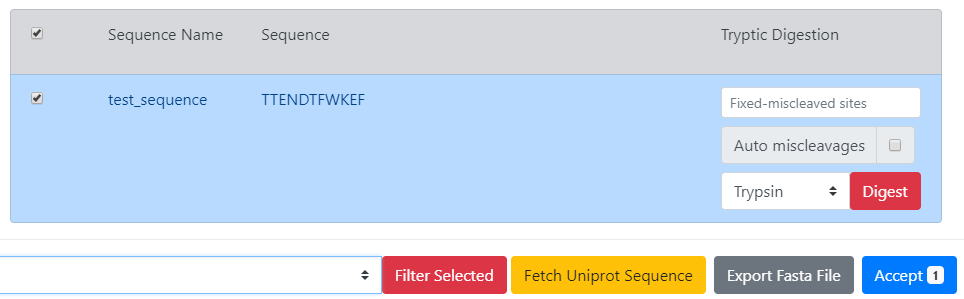
\includegraphics{test-sequence-ylibrary}
		\end{adjustbox}
		\caption{Example sequence input.}\label{fig:testsequenceylibrary}
	\end{framed}
\end{figure}


This sequence has an N-glycosylation sequon at position 4 and a tryptic digestion site right after position 9. With this library, we aimed to generate all HexNAc Y0, Y1, and Y2 transitions for the sequence at RT of 10 across all SWATH windows. The max charge allowed would be 2 and the annotated sequence at the modification position would include both RT and SWATH window value.\par


After in-silico digestion with trypsin, we would obtain two sequences (Figure \ref{fig:testsequenceylibrarydigested}), one before and one after the digestion site. The name of the sequences have also been automatically modified to show the starting and stopping positions of each digested fragment. Using the filter rule for N-glycosylation sequon, the GUI would identify and select all sequences with a sequon within those already selected.
\begin{figure}[H]
	\centering
	\begin{framed}
        \centering
        \begin{adjustbox}{width=1\textwidth}
			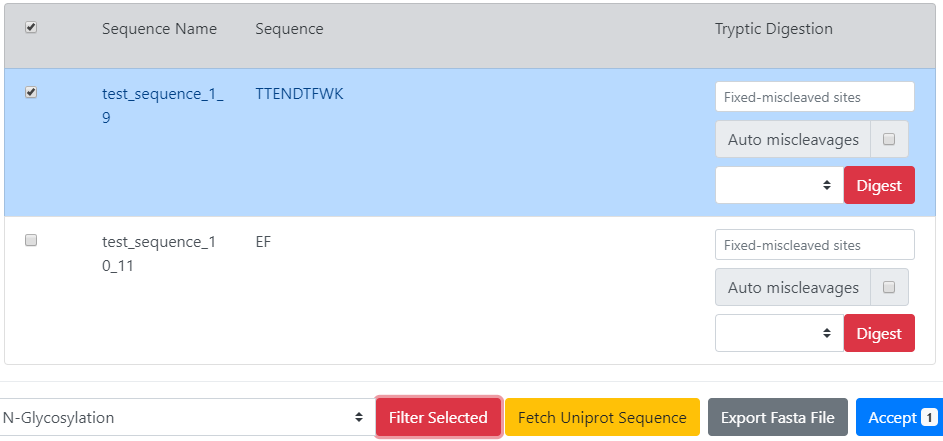
\includegraphics{test-sequence-ylibrary-digested}
		\end{adjustbox}
		\caption{Example sequence input after in-silico trypsin digestion and filtered for only those containing N-glycosylation sequon.}\label{fig:testsequenceylibrarydigested}
	\end{framed}
\end{figure}

We currently have a tryptic digested sequence containing N-glycosylation sequon but without any modification and experiment settings applied to it. These settings can be selected within the \textbf{Queryset Input Settings} panel.

In Figure \ref{fig:testsequenceylibrarysettings}, we have the following settings selected,
\begin{itemize}
	\item HexNAc Y0, Y1, and Y2 modifications.
	\item Retention time at 10.
	\item All SWATH windows.
	\item Y fragmentation ion-type
	\item Output sequence format include RT and SWATH window values at variable modification sites.
\end{itemize}
\begin{figure}[H]
	\centering
	\begin{framed}
        \centering
        \begin{adjustbox}{width=1\textwidth}
			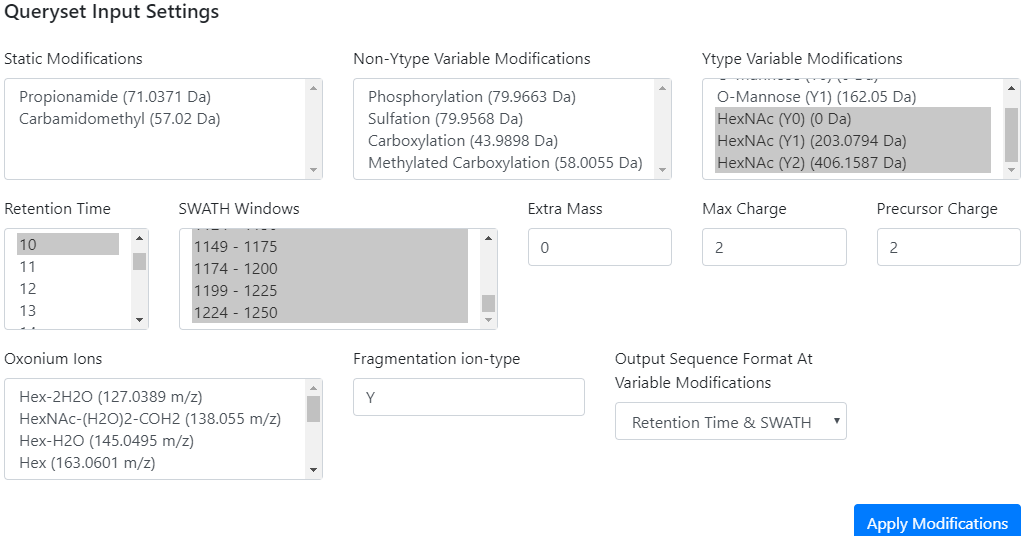
\includegraphics{test-sequence-ylibrary-settings}
		\end{adjustbox}
		\caption{Example modification settings for N-glycosylation library with 3 HexNAc Ytype transitions at RT 10 and across all default SWATH windows.}\label{fig:testsequenceylibrarysettings}
	\end{framed}
\end{figure}
After application of modification settings, the result would be similar to Figure \ref{fig:testsequenceylibraryindividual}. Multiple HexNAc transitions are placed at N4 and the residue is colored green.
\begin{figure}[H]
	\centering
	\begin{framed}
        \centering
        \begin{adjustbox}{width=1\textwidth}
			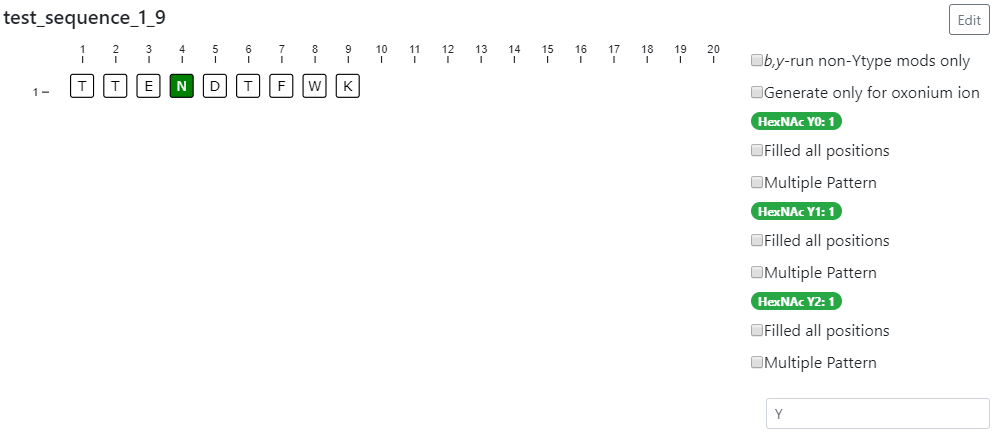
\includegraphics{test-sequence-ylibrary-individual}
		\end{adjustbox}
		\caption{Example of a sequence with the settings above applied.}\label{fig:testsequenceylibraryindividual}
	\end{framed}
\end{figure}

On submission, the progress bar would start. When a query is finished, the bar under it would turn green. The moment all queries result have finished and been collected, a \textbf{Save Compiled Results} button would appear under the \textbf{Submit Queries} button. The user can click on the button to save the library in .txt tabulated file format.

\subsection{Creating a byY-library}
For a library with both \emph{by} and \emph{Y} transitions, the user might want to avoid overlapping of the transition m/z, especially \emph{y} and \emph{Y} transitions. The \textbf{b,y-run non-Ytype mods only} option can be enabled for the query. This option would disable Ytype modification mass within calculation of transition m/z for \emph{by}-series.

\section{Adding oxonium ions to Y-library}
In MS data of glycosylated peptides, Oxonium ions are fragmentation of the modification block during ionization process. The presence of oxonium ions fragment within the spectral graph of a peptide fragment could provide additional evidence for the peptide to be glycosylation and potential knowledge on the glycan composition. With SWATHLib, using the query settings interface, you can add these oxonium ions to your library of interests to look for potential glycosylation evidence.\par

Let start again with the example sequence from the section above.\par
\begin{verbatim}
	>test_sequence
	TTENDTFWKEF
\end{verbatim}

Following similar input procedure as of Figure \ref{fig:testsequenceylibrarysettings} we would obtain the digested peptide containing at least one N-glycosylation sequon. However, different to what depicted previously, our settings would now include the oxonium ions Hex, HexNAc, and HexHexNAc.\par

\begin{figure}[H]
	\centering
	\begin{framed}
        \centering
        \begin{adjustbox}{width=1\textwidth}
			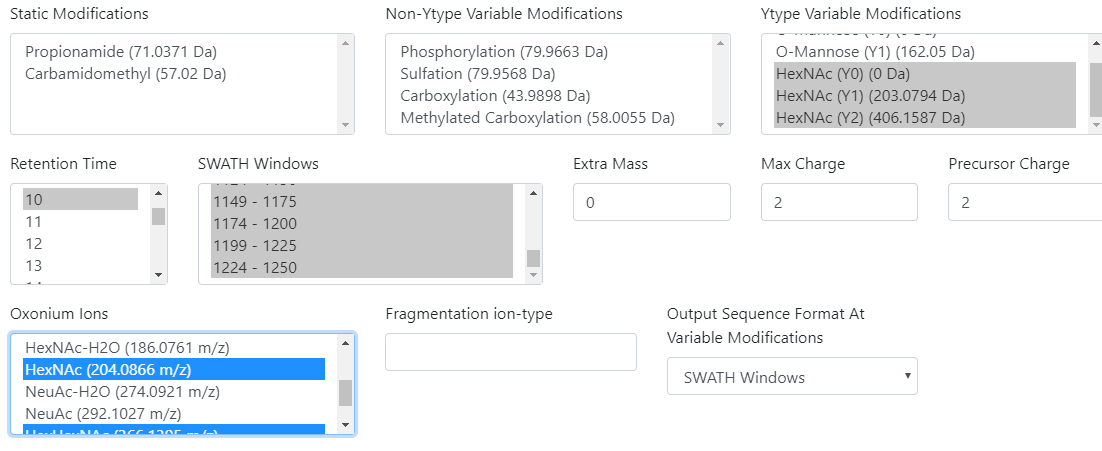
\includegraphics{test-sequence-yoxoniumlibrary-settings}
		\end{adjustbox}
		\caption{Example of a sequence with the oxonium ions selected. By selecting these settings, every single modified variation of the peptide at each selected window and retention time would also be accompanied by entries of selected oxonium ions.}\label{fig:testsequenceyoxoniumlibrarysettings}
	\end{framed}
\end{figure}

These settings together with the query can now be submitted for process to produce a library with Y-ion together with those selected oxonium ions.\par

\subsection{Oxoniome library}
An oxoniome library is one that containing only oxonium ions. It can be used to quickly gain an overview of glycosylation within complex samples. SWATHLib can be used to create an oxoniome library from peptide of interests. 

\begin{figure}[H]
	\centering
	\begin{framed}
        \centering
        \begin{adjustbox}{width=1\textwidth}
			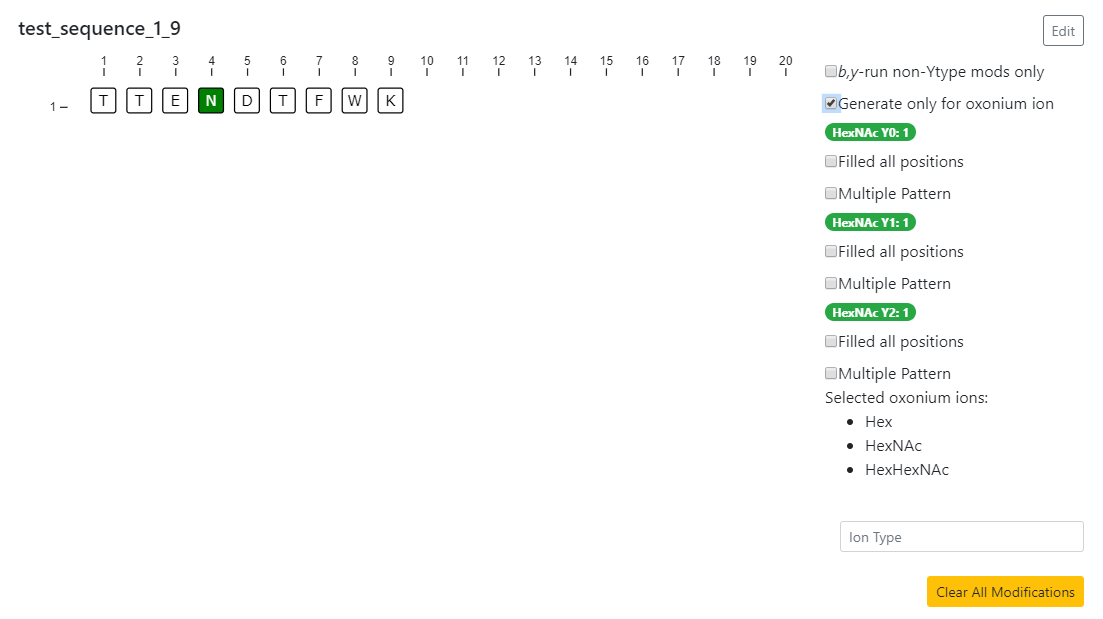
\includegraphics{test-sequence-yoxoniumlibrary-individual}
		\end{adjustbox}
		\caption{Example of a sequence with the oxonium ions selected and is set for only oxonium generation.}\label{fig:testsequenceyoxoniumlibraryindividual}
	\end{framed}
\end{figure}

In Figure \ref{fig:testsequenceyoxoniumlibraryindividual}, the option \textbf{Generate only for oxonium ion} was checked to instruct the back-end only generating oxonium ions entry for each modification pattern without calculating any \emph{Y} or \emph{by}-transitions. Currently this setting is only available on an individual sequence basic. The sequence and all modifications input would only be used to identify different modification pattern of the input peptides.\par

SWATHLib can also generate oxoniome library for arbitrary peptides as long as no modifications and transitions are put on the arbitrary peptides in the settings.\par
\end{document}